\documentclass[1p]{elsarticle_modified}
%\bibliographystyle{elsarticle-num}

%\usepackage[colorlinks]{hyperref}
%\usepackage{abbrmath_seonhwa} %\Abb, \Ascr, \Acal ,\Abf, \Afrak
\usepackage{amsfonts}
\usepackage{amssymb}
\usepackage{amsmath}
\usepackage{amsthm}
\usepackage{scalefnt}
\usepackage{amsbsy}
\usepackage{kotex}
\usepackage{caption}
\usepackage{subfig}
\usepackage{color}
\usepackage{graphicx}
\usepackage{xcolor} %% white, black, red, green, blue, cyan, magenta, yellow
\usepackage{float}
\usepackage{setspace}
\usepackage{hyperref}

\usepackage{tikz}
\usetikzlibrary{arrows}

\usepackage{multirow}
\usepackage{array} % fixed length table
\usepackage{hhline}

%%%%%%%%%%%%%%%%%%%%%
\makeatletter
\renewcommand*\env@matrix[1][\arraystretch]{%
	\edef\arraystretch{#1}%
	\hskip -\arraycolsep
	\let\@ifnextchar\new@ifnextchar
	\array{*\c@MaxMatrixCols c}}
\makeatother %https://tex.stackexchange.com/questions/14071/how-can-i-increase-the-line-spacing-in-a-matrix
%%%%%%%%%%%%%%%

\usepackage[normalem]{ulem}

\newcommand{\msout}[1]{\ifmmode\text{\sout{\ensuremath{#1}}}\else\sout{#1}\fi}
%SOURCE: \msout is \stkout macro in https://tex.stackexchange.com/questions/20609/strikeout-in-math-mode

\newcommand{\cancel}[1]{
	\ifmmode
	{\color{red}\msout{#1}}
	\else
	{\color{red}\sout{#1}}
	\fi
}

\newcommand{\add}[1]{
	{\color{blue}\uwave{#1}}
}

\newcommand{\replace}[2]{
	\ifmmode
	{\color{red}\msout{#1}}{\color{blue}\uwave{#2}}
	\else
	{\color{red}\sout{#1}}{\color{blue}\uwave{#2}}
	\fi
}

\newcommand{\Sol}{\mathcal{S}} %segment
\newcommand{\D}{D} %diagram
\newcommand{\A}{\mathcal{A}} %arc


%%%%%%%%%%%%%%%%%%%%%%%%%%%%%5 test

\def\sl{\operatorname{\textup{SL}}(2,\Cbb)}
\def\psl{\operatorname{\textup{PSL}}(2,\Cbb)}
\def\quan{\mkern 1mu \triangleright \mkern 1mu}

\theoremstyle{definition}
\newtheorem{thm}{Theorem}[section]
\newtheorem{prop}[thm]{Proposition}
\newtheorem{lem}[thm]{Lemma}
\newtheorem{ques}[thm]{Question}
\newtheorem{cor}[thm]{Corollary}
\newtheorem{defn}[thm]{Definition}
\newtheorem{exam}[thm]{Example}
\newtheorem{rmk}[thm]{Remark}
\newtheorem{alg}[thm]{Algorithm}

\newcommand{\I}{\sqrt{-1}}
\begin{document}

%\begin{frontmatter}
%
%\title{Boundary parabolic representations of knots up to 8 crossings}
%
%%% Group authors per affiliation:
%\author{Yunhi Cho} 
%\address{Department of Mathematics, University of Seoul, Seoul, Korea}
%\ead{yhcho@uos.ac.kr}
%
%
%\author{Seonhwa Kim} %\fnref{s_kim}}
%\address{Center for Geometry and Physics, Institute for Basic Science, Pohang, 37673, Korea}
%\ead{ryeona17@ibs.re.kr}
%
%\author{Hyuk Kim}
%\address{Department of Mathematical Sciences, Seoul National University, Seoul 08826, Korea}
%\ead{hyukkim@snu.ac.kr}
%
%\author{Seokbeom Yoon}
%\address{Department of Mathematical Sciences, Seoul National University, Seoul, 08826,  Korea}
%\ead{sbyoon15@snu.ac.kr}
%
%\begin{abstract}
%We find all boundary parabolic representation of knots up to 8 crossings.
%
%\end{abstract}
%\begin{keyword}
%    \MSC[2010] 57M25 
%\end{keyword}
%
%\end{frontmatter}

%\linenumbers
%\tableofcontents
%
\newcommand\colored[1]{\textcolor{white}{\rule[-0.35ex]{0.8em}{1.4ex}}\kern-0.8em\color{red} #1}%
%\newcommand\colored[1]{\textcolor{white}{ #1}\kern-2.17ex	\textcolor{white}{ #1}\kern-1.81ex	\textcolor{white}{ #1}\kern-2.15ex\color{red}#1	}

{\Large $\underline{12a_{1208}~(K12a_{1208})}$}

\setlength{\tabcolsep}{10pt}
\renewcommand{\arraystretch}{1.6}
\vspace{1cm}\begin{tabular}{m{100pt}>{\centering\arraybackslash}m{274pt}}
\multirow{5}{120pt}{
	\centering
	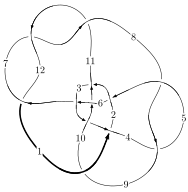
\includegraphics[width=112pt]{../../../GIT/diagram.site/Diagrams/png/2009_12a_1208.png}\\
\ \ \ A knot diagram\footnotemark}&
\allowdisplaybreaks
\textbf{Linearized knot diagam} \\
\cline{2-2}
 &
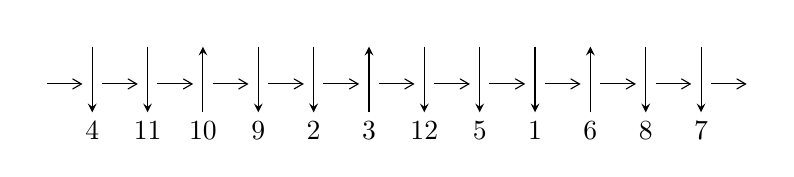
\begin{tikzpicture}[x=20pt, y=17pt]
	% nodes
	\node (C0) at (0, 0) {};
	\node (C1) at (1, 0) {};
	\node (C1U) at (1, +1) {};
	\node (C1D) at (1, -1) {4};

	\node (C2) at (2, 0) {};
	\node (C2U) at (2, +1) {};
	\node (C2D) at (2, -1) {11};

	\node (C3) at (3, 0) {};
	\node (C3U) at (3, +1) {};
	\node (C3D) at (3, -1) {10};

	\node (C4) at (4, 0) {};
	\node (C4U) at (4, +1) {};
	\node (C4D) at (4, -1) {9};

	\node (C5) at (5, 0) {};
	\node (C5U) at (5, +1) {};
	\node (C5D) at (5, -1) {2};

	\node (C6) at (6, 0) {};
	\node (C6U) at (6, +1) {};
	\node (C6D) at (6, -1) {3};

	\node (C7) at (7, 0) {};
	\node (C7U) at (7, +1) {};
	\node (C7D) at (7, -1) {12};

	\node (C8) at (8, 0) {};
	\node (C8U) at (8, +1) {};
	\node (C8D) at (8, -1) {5};

	\node (C9) at (9, 0) {};
	\node (C9U) at (9, +1) {};
	\node (C9D) at (9, -1) {1};

	\node (C10) at (10, 0) {};
	\node (C10U) at (10, +1) {};
	\node (C10D) at (10, -1) {6};

	\node (C11) at (11, 0) {};
	\node (C11U) at (11, +1) {};
	\node (C11D) at (11, -1) {8};

	\node (C12) at (12, 0) {};
	\node (C12U) at (12, +1) {};
	\node (C12D) at (12, -1) {7};
	\node (C13) at (13, 0) {};

	% arrows
	\draw[->,>={angle 60}]
	(C0) edge (C1) (C1) edge (C2) (C2) edge (C3) (C3) edge (C4) (C4) edge (C5) (C5) edge (C6) (C6) edge (C7) (C7) edge (C8) (C8) edge (C9) (C9) edge (C10) (C10) edge (C11) (C11) edge (C12) (C12) edge (C13) ;	\draw[->,>=stealth]
	(C1U) edge (C1D) (C2U) edge (C2D) (C3D) edge (C3U) (C4U) edge (C4D) (C5U) edge (C5D) (C6D) edge (C6U) (C7U) edge (C7D) (C8U) edge (C8D) (C9U) edge (C9D) (C10D) edge (C10U) (C11U) edge (C11D) (C12U) edge (C12D) ;
	\end{tikzpicture} \\
\hhline{~~} \\& 
\textbf{Solving Sequence} \\ \cline{2-2} 
 &
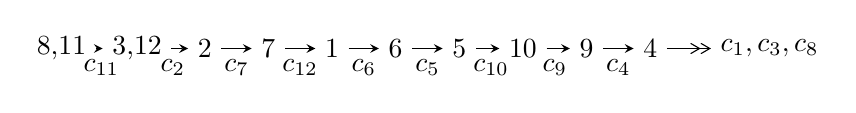
\begin{tikzpicture}[x=23pt, y=7pt]
	% node
	\node (A0) at (-1/8, 0) {8,11};
	\node (A1) at (17/16, 0) {3,12};
	\node (A2) at (17/8, 0) {2};
	\node (A3) at (25/8, 0) {7};
	\node (A4) at (33/8, 0) {1};
	\node (A5) at (41/8, 0) {6};
	\node (A6) at (49/8, 0) {5};
	\node (A7) at (57/8, 0) {10};
	\node (A8) at (65/8, 0) {9};
	\node (A9) at (73/8, 0) {4};
	\node (C1) at (1/2, -1) {$c_{11}$};
	\node (C2) at (13/8, -1) {$c_{2}$};
	\node (C3) at (21/8, -1) {$c_{7}$};
	\node (C4) at (29/8, -1) {$c_{12}$};
	\node (C5) at (37/8, -1) {$c_{6}$};
	\node (C6) at (45/8, -1) {$c_{5}$};
	\node (C7) at (53/8, -1) {$c_{10}$};
	\node (C8) at (61/8, -1) {$c_{9}$};
	\node (C9) at (69/8, -1) {$c_{4}$};
	\node (A10) at (11, 0) {$c_{1},c_{3},c_{8}$};

	% edge
	\draw[->,>=stealth]	
	(A0) edge (A1) (A1) edge (A2) (A2) edge (A3) (A3) edge (A4) (A4) edge (A5) (A5) edge (A6) (A6) edge (A7) (A7) edge (A8) (A8) edge (A9) ;
	\draw[->>,>={angle 60}]	
	(A9) edge (A10);
\end{tikzpicture} \\ 

\end{tabular} \\

\footnotetext{
The image of knot diagram is generated by the software ``\textbf{Draw programme}" developed by Andrew Bartholomew(\url{http://www.layer8.co.uk/maths/draw/index.htm\#Running-draw}), where we modified some parts for our purpose(\url{https://github.com/CATsTAILs/LinksPainter}).
}\phantom \\ \newline 
\centering \textbf{Ideals for irreducible components\footnotemark of $X_{\text{par}}$} 
 
\begin{align*}
I^u_{1}&=\langle 
2.07625\times10^{594} u^{165}+5.47091\times10^{594} u^{164}+\cdots+1.02629\times10^{595} b+3.00733\times10^{596},\\
\phantom{I^u_{1}}&\phantom{= \langle  }-3.37299\times10^{595} u^{165}+2.18527\times10^{596} u^{164}+\cdots+8.72344\times10^{596} a+4.06613\times10^{598},\\
\phantom{I^u_{1}}&\phantom{= \langle  }u^{166}+2 u^{165}+\cdots-714 u+289\rangle \\
I^u_{2}&=\langle 
1355679442634 u^{42}-1138023218267 u^{41}+\cdots+286979954013 b-2810619597407,\\
\phantom{I^u_{2}}&\phantom{= \langle  }-190977593434 u^{42}+27758049080035 u^{41}+\cdots+860939862039 a+32882509966417,\\
\phantom{I^u_{2}}&\phantom{= \langle  }u^{43}+u^{42}+\cdots+10 u+1\rangle \\
\\
\end{align*}
\raggedright * 2 irreducible components of $\dim_{\mathbb{C}}=0$, with total 209 representations.\\
\footnotetext{All coefficients of polynomials are rational numbers. But the coefficients are sometimes approximated in decimal forms when there is not enough margin.}
\newpage
\renewcommand{\arraystretch}{1}
\centering \section*{I. $I^u_{1}= \langle 2.08\times10^{594} u^{165}+5.47\times10^{594} u^{164}+\cdots+1.03\times10^{595} b+3.01\times10^{596},\;-3.37\times10^{595} u^{165}+2.19\times10^{596} u^{164}+\cdots+8.72\times10^{596} a+4.07\times10^{598},\;u^{166}+2 u^{165}+\cdots-714 u+289 \rangle$}
\flushleft \textbf{(i) Arc colorings}\\
\begin{tabular}{m{7pt} m{180pt} m{7pt} m{180pt} }
\flushright $a_{8}=$&$\begin{pmatrix}0\\u\end{pmatrix}$ \\
\flushright $a_{11}=$&$\begin{pmatrix}1\\0\end{pmatrix}$ \\
\flushright $a_{3}=$&$\begin{pmatrix}0.0386659 u^{165}-0.250505 u^{164}+\cdots+103.290 u-46.6115\\-0.202307 u^{165}-0.533078 u^{164}+\cdots+34.8210 u-29.3030\end{pmatrix}$ \\
\flushright $a_{12}=$&$\begin{pmatrix}1\\u^2\end{pmatrix}$ \\
\flushright $a_{2}=$&$\begin{pmatrix}-0.163641 u^{165}-0.783583 u^{164}+\cdots+138.111 u-75.9146\\-0.202307 u^{165}-0.533078 u^{164}+\cdots+34.8210 u-29.3030\end{pmatrix}$ \\
\flushright $a_{7}=$&$\begin{pmatrix}u\\u^3+u\end{pmatrix}$ \\
\flushright $a_{1}=$&$\begin{pmatrix}u^2+1\\u^4+2 u^2\end{pmatrix}$ \\
\flushright $a_{6}=$&$\begin{pmatrix}-1.21009 u^{165}-3.04394 u^{164}+\cdots-37.7098 u-83.1115\\-0.0751152 u^{165}-0.524075 u^{164}+\cdots+127.144 u-55.8265\end{pmatrix}$ \\
\flushright $a_{5}=$&$\begin{pmatrix}0.277604 u^{165}+0.563644 u^{164}+\cdots+54.4908 u-3.35099\\-1.15054 u^{165}-3.71939 u^{164}+\cdots+435.410 u-255.120\end{pmatrix}$ \\
\flushright $a_{10}=$&$\begin{pmatrix}0.482406 u^{165}-0.333118 u^{164}+\cdots+660.458 u-236.350\\-0.537254 u^{165}-0.742007 u^{164}+\cdots-231.635 u+55.4828\end{pmatrix}$ \\
\flushright $a_{9}=$&$\begin{pmatrix}0.0940036 u^{165}-0.413368 u^{164}+\cdots+290.152 u-113.207\\-0.869761 u^{165}-0.726677 u^{164}+\cdots-586.984 u+175.849\end{pmatrix}$ \\
\flushright $a_{4}=$&$\begin{pmatrix}-0.0760578 u^{165}-0.388130 u^{164}+\cdots+98.5661 u-50.4660\\-0.665368 u^{165}-1.81042 u^{164}+\cdots+115.272 u-91.2676\end{pmatrix}$\\&\end{tabular}
\flushleft \textbf{(ii) Obstruction class $= -1$}\\~\\
\flushleft \textbf{(iii) Cusp Shapes $= 1.84451 u^{165}+4.84351 u^{164}+\cdots-35.4126 u+139.634$}\\~\\
\newpage\renewcommand{\arraystretch}{1}
\flushleft \textbf{(iv) u-Polynomials at the component}\newline \\
\begin{tabular}{m{50pt}|m{274pt}}
Crossings & \hspace{64pt}u-Polynomials at each crossing \\
\hline $$\begin{aligned}c_{1}\end{aligned}$$&$\begin{aligned}
&u^{166}+15 u^{165}+\cdots+14 u-1
\end{aligned}$\\
\hline $$\begin{aligned}c_{2}\end{aligned}$$&$\begin{aligned}
&u^{166}-4 u^{165}+\cdots+28476 u+667
\end{aligned}$\\
\hline $$\begin{aligned}c_{3}\end{aligned}$$&$\begin{aligned}
&u^{166}-3 u^{165}+\cdots-8268033 u+335191
\end{aligned}$\\
\hline $$\begin{aligned}c_{4},c_{8}\end{aligned}$$&$\begin{aligned}
&u^{166}- u^{165}+\cdots-228154 u+191449
\end{aligned}$\\
\hline $$\begin{aligned}c_{5}\end{aligned}$$&$\begin{aligned}
&u^{166}-2 u^{165}+\cdots+2701472 u-273472
\end{aligned}$\\
\hline $$\begin{aligned}c_{6}\end{aligned}$$&$\begin{aligned}
&u^{166}-10 u^{165}+\cdots+634 u-109
\end{aligned}$\\
\hline $$\begin{aligned}c_{7},c_{11},c_{12}\end{aligned}$$&$\begin{aligned}
&u^{166}+2 u^{165}+\cdots-714 u+289
\end{aligned}$\\
\hline $$\begin{aligned}c_{9}\end{aligned}$$&$\begin{aligned}
&u^{166}- u^{165}+\cdots-67072 u+22016
\end{aligned}$\\
\hline $$\begin{aligned}c_{10}\end{aligned}$$&$\begin{aligned}
&u^{166}+5 u^{165}+\cdots-15 u+1
\end{aligned}$\\
\hline
\end{tabular}\\~\\
\newpage\renewcommand{\arraystretch}{1}
\flushleft \textbf{(v) Riley Polynomials at the component}\newline \\
\begin{tabular}{m{50pt}|m{274pt}}
Crossings & \hspace{64pt}Riley Polynomials at each crossing \\
\hline $$\begin{aligned}c_{1}\end{aligned}$$&$\begin{aligned}
&y^{166}+y^{165}+\cdots-14 y+1
\end{aligned}$\\
\hline $$\begin{aligned}c_{2}\end{aligned}$$&$\begin{aligned}
&y^{166}-2 y^{165}+\cdots-1188891486 y+444889
\end{aligned}$\\
\hline $$\begin{aligned}c_{3}\end{aligned}$$&$\begin{aligned}
&y^{166}+61 y^{165}+\cdots-3152875669969 y+112353006481
\end{aligned}$\\
\hline $$\begin{aligned}c_{4},c_{8}\end{aligned}$$&$\begin{aligned}
&y^{166}+117 y^{165}+\cdots+1929765685298 y+36652719601
\end{aligned}$\\
\hline $$\begin{aligned}c_{5}\end{aligned}$$&$\begin{aligned}
&y^{166}-30 y^{165}+\cdots-5537587637248 y+74786934784
\end{aligned}$\\
\hline $$\begin{aligned}c_{6}\end{aligned}$$&$\begin{aligned}
&y^{166}+18 y^{165}+\cdots-1172586 y+11881
\end{aligned}$\\
\hline $$\begin{aligned}c_{7},c_{11},c_{12}\end{aligned}$$&$\begin{aligned}
&y^{166}+158 y^{165}+\cdots+2222988 y+83521
\end{aligned}$\\
\hline $$\begin{aligned}c_{9}\end{aligned}$$&$\begin{aligned}
&y^{166}+21 y^{165}+\cdots+28523233280 y+484704256
\end{aligned}$\\
\hline $$\begin{aligned}c_{10}\end{aligned}$$&$\begin{aligned}
&y^{166}+15 y^{165}+\cdots-249 y+1
\end{aligned}$\\
\hline
\end{tabular}\\~\\
\newpage\flushleft \textbf{(vi) Complex Volumes and Cusp Shapes}
$$\begin{array}{c|c|c}  
\text{Solutions to }I^u_{1}& \I (\text{vol} + \sqrt{-1}CS) & \text{Cusp shape}\\
 \hline 
\begin{aligned}
u &= -0.725948 + 0.683647 I \\
a &= -0.038423 + 0.619652 I \\
b &= \phantom{-}0.256542 - 0.112019 I\end{aligned}
 & \phantom{-}0.02086 + 2.75664 I & \phantom{-0.000000 } 0 \\ \hline\begin{aligned}
u &= -0.725948 - 0.683647 I \\
a &= -0.038423 - 0.619652 I \\
b &= \phantom{-}0.256542 + 0.112019 I\end{aligned}
 & \phantom{-}0.02086 - 2.75664 I & \phantom{-0.000000 } 0 \\ \hline\begin{aligned}
u &= \phantom{-}0.025517 + 0.986919 I \\
a &= -1.110390 + 0.549998 I \\
b &= \phantom{-}1.104750 - 0.503162 I\end{aligned}
 & \phantom{-}0.89681 + 3.77593 I & \phantom{-0.000000 } 0 \\ \hline\begin{aligned}
u &= \phantom{-}0.025517 - 0.986919 I \\
a &= -1.110390 - 0.549998 I \\
b &= \phantom{-}1.104750 + 0.503162 I\end{aligned}
 & \phantom{-}0.89681 - 3.77593 I & \phantom{-0.000000 } 0 \\ \hline\begin{aligned}
u &= -0.946801 + 0.396249 I \\
a &= \phantom{-}0.734629 + 0.455554 I \\
b &= \phantom{-}1.01961 - 1.14872 I\end{aligned}
 & \phantom{-}0.4546 + 15.7472 I & \phantom{-0.000000 } 0 \\ \hline\begin{aligned}
u &= -0.946801 - 0.396249 I \\
a &= \phantom{-}0.734629 - 0.455554 I \\
b &= \phantom{-}1.01961 + 1.14872 I\end{aligned}
 & \phantom{-}0.4546 - 15.7472 I & \phantom{-0.000000 } 0 \\ \hline\begin{aligned}
u &= -0.794890 + 0.511199 I \\
a &= -0.292218 + 0.368860 I \\
b &= \phantom{-}0.467134 + 0.346393 I\end{aligned}
 & -3.38316 + 0.71507 I & \phantom{-0.000000 } 0 \\ \hline\begin{aligned}
u &= -0.794890 - 0.511199 I \\
a &= -0.292218 - 0.368860 I \\
b &= \phantom{-}0.467134 - 0.346393 I\end{aligned}
 & -3.38316 - 0.71507 I & \phantom{-0.000000 } 0 \\ \hline\begin{aligned}
u &= \phantom{-}1.049290 + 0.235908 I \\
a &= \phantom{-}0.301042 + 0.002024 I \\
b &= \phantom{-}0.316727 + 0.503949 I\end{aligned}
 & \phantom{-}1.78942 - 6.85416 I & \phantom{-0.000000 } 0 \\ \hline\begin{aligned}
u &= \phantom{-}1.049290 - 0.235908 I \\
a &= \phantom{-}0.301042 - 0.002024 I \\
b &= \phantom{-}0.316727 - 0.503949 I\end{aligned}
 & \phantom{-}1.78942 + 6.85416 I & \phantom{-0.000000 } 0\\
 \hline 
 \end{array}$$\newpage$$\begin{array}{c|c|c}  
\text{Solutions to }I^u_{1}& \I (\text{vol} + \sqrt{-1}CS) & \text{Cusp shape}\\
 \hline 
\begin{aligned}
u &= \phantom{-}0.556720 + 0.733265 I \\
a &= \phantom{-}0.525878 + 0.156768 I \\
b &= -0.909625 + 0.665707 I\end{aligned}
 & -2.58532 + 5.21679 I & \phantom{-0.000000 } 0 \\ \hline\begin{aligned}
u &= \phantom{-}0.556720 - 0.733265 I \\
a &= \phantom{-}0.525878 - 0.156768 I \\
b &= -0.909625 - 0.665707 I\end{aligned}
 & -2.58532 - 5.21679 I & \phantom{-0.000000 } 0 \\ \hline\begin{aligned}
u &= \phantom{-}0.600379 + 0.688416 I \\
a &= -0.534562 - 0.328227 I \\
b &= -0.439443 - 0.877361 I\end{aligned}
 & -1.60622 - 2.48356 I & \phantom{-0.000000 } 0 \\ \hline\begin{aligned}
u &= \phantom{-}0.600379 - 0.688416 I \\
a &= -0.534562 + 0.328227 I \\
b &= -0.439443 + 0.877361 I\end{aligned}
 & -1.60622 + 2.48356 I & \phantom{-0.000000 } 0 \\ \hline\begin{aligned}
u &= \phantom{-}0.369614 + 1.033310 I \\
a &= \phantom{-}0.131564 - 0.169829 I \\
b &= \phantom{-}0.290813 + 0.632611 I\end{aligned}
 & \phantom{-}4.88400 + 1.56084 I & \phantom{-0.000000 } 0 \\ \hline\begin{aligned}
u &= \phantom{-}0.369614 - 1.033310 I \\
a &= \phantom{-}0.131564 + 0.169829 I \\
b &= \phantom{-}0.290813 - 0.632611 I\end{aligned}
 & \phantom{-}4.88400 - 1.56084 I & \phantom{-0.000000 } 0 \\ \hline\begin{aligned}
u &= -0.132622 + 1.117560 I \\
a &= \phantom{-}1.24662 + 0.98339 I \\
b &= -0.703852 + 0.079105 I\end{aligned}
 & \phantom{-}4.07151 + 6.08335 I & \phantom{-0.000000 } 0 \\ \hline\begin{aligned}
u &= -0.132622 - 1.117560 I \\
a &= \phantom{-}1.24662 - 0.98339 I \\
b &= -0.703852 - 0.079105 I\end{aligned}
 & \phantom{-}4.07151 - 6.08335 I & \phantom{-0.000000 } 0 \\ \hline\begin{aligned}
u &= \phantom{-}0.788182 + 0.368170 I \\
a &= \phantom{-}0.782020 - 0.769821 I \\
b &= \phantom{-}1.048490 + 0.884888 I\end{aligned}
 & -3.77502 - 9.90973 I & \phantom{-0.000000 } 0 \\ \hline\begin{aligned}
u &= \phantom{-}0.788182 - 0.368170 I \\
a &= \phantom{-}0.782020 + 0.769821 I \\
b &= \phantom{-}1.048490 - 0.884888 I\end{aligned}
 & -3.77502 + 9.90973 I & \phantom{-0.000000 } 0\\
 \hline 
 \end{array}$$\newpage$$\begin{array}{c|c|c}  
\text{Solutions to }I^u_{1}& \I (\text{vol} + \sqrt{-1}CS) & \text{Cusp shape}\\
 \hline 
\begin{aligned}
u &= -0.554858 + 0.666692 I \\
a &= -0.095827 - 0.534005 I \\
b &= -0.826350 + 0.668994 I\end{aligned}
 & -2.76581 + 4.07346 I & \phantom{-0.000000 } 0 \\ \hline\begin{aligned}
u &= -0.554858 - 0.666692 I \\
a &= -0.095827 + 0.534005 I \\
b &= -0.826350 - 0.668994 I\end{aligned}
 & -2.76581 - 4.07346 I & \phantom{-0.000000 } 0 \\ \hline\begin{aligned}
u &= -0.405250 + 0.744541 I \\
a &= -0.632404 + 0.871648 I \\
b &= \phantom{-}0.588314 + 0.139635 I\end{aligned}
 & -0.11721 + 2.83841 I & \phantom{-0.000000 } 0 \\ \hline\begin{aligned}
u &= -0.405250 - 0.744541 I \\
a &= -0.632404 - 0.871648 I \\
b &= \phantom{-}0.588314 - 0.139635 I\end{aligned}
 & -0.11721 - 2.83841 I & \phantom{-0.000000 } 0 \\ \hline\begin{aligned}
u &= -0.732834 + 0.338965 I \\
a &= -1.195570 - 0.003043 I \\
b &= -0.113109 + 0.305420 I\end{aligned}
 & \phantom{-}2.24288 - 2.77835 I & \phantom{-0.000000 } 0 \\ \hline\begin{aligned}
u &= -0.732834 - 0.338965 I \\
a &= -1.195570 + 0.003043 I \\
b &= -0.113109 - 0.305420 I\end{aligned}
 & \phantom{-}2.24288 + 2.77835 I & \phantom{-0.000000 } 0 \\ \hline\begin{aligned}
u &= -0.053658 + 1.192690 I \\
a &= \phantom{-}0.58502 + 3.52803 I \\
b &= \phantom{-}0.01778 - 1.61639 I\end{aligned}
 & \phantom{-}1.35245 + 6.33268 I & \phantom{-0.000000 } 0 \\ \hline\begin{aligned}
u &= -0.053658 - 1.192690 I \\
a &= \phantom{-}0.58502 - 3.52803 I \\
b &= \phantom{-}0.01778 + 1.61639 I\end{aligned}
 & \phantom{-}1.35245 - 6.33268 I & \phantom{-0.000000 } 0 \\ \hline\begin{aligned}
u &= -0.336940 + 0.717872 I \\
a &= -0.652905 + 1.059580 I \\
b &= \phantom{-}0.833983 - 0.388471 I\end{aligned}
 & \phantom{-}0.97295 + 3.91183 I & \phantom{-0.000000 } 0 \\ \hline\begin{aligned}
u &= -0.336940 - 0.717872 I \\
a &= -0.652905 - 1.059580 I \\
b &= \phantom{-}0.833983 + 0.388471 I\end{aligned}
 & \phantom{-}0.97295 - 3.91183 I & \phantom{-0.000000 } 0\\
 \hline 
 \end{array}$$\newpage$$\begin{array}{c|c|c}  
\text{Solutions to }I^u_{1}& \I (\text{vol} + \sqrt{-1}CS) & \text{Cusp shape}\\
 \hline 
\begin{aligned}
u &= \phantom{-}0.785466 + 0.089428 I \\
a &= -1.22500 + 0.71118 I \\
b &= -1.006870 - 0.678413 I\end{aligned}
 & -1.30016 - 4.36479 I & \phantom{-0.000000 } 0 \\ \hline\begin{aligned}
u &= \phantom{-}0.785466 - 0.089428 I \\
a &= -1.22500 - 0.71118 I \\
b &= -1.006870 + 0.678413 I\end{aligned}
 & -1.30016 + 4.36479 I & \phantom{-0.000000 } 0 \\ \hline\begin{aligned}
u &= -0.793606 + 0.916192 I \\
a &= \phantom{-}0.550045 - 0.061150 I \\
b &= -0.745314 - 1.088650 I\end{aligned}
 & \phantom{-}1.92998 - 9.84732 I & \phantom{-0.000000 } 0 \\ \hline\begin{aligned}
u &= -0.793606 - 0.916192 I \\
a &= \phantom{-}0.550045 + 0.061150 I \\
b &= -0.745314 + 1.088650 I\end{aligned}
 & \phantom{-}1.92998 + 9.84732 I & \phantom{-0.000000 } 0 \\ \hline\begin{aligned}
u &= -0.040204 + 1.222260 I \\
a &= -1.76830 + 0.36131 I \\
b &= \phantom{-}1.65751 - 0.03653 I\end{aligned}
 & \phantom{-}0.54565 + 1.96085 I & \phantom{-0.000000 } 0 \\ \hline\begin{aligned}
u &= -0.040204 - 1.222260 I \\
a &= -1.76830 - 0.36131 I \\
b &= \phantom{-}1.65751 + 0.03653 I\end{aligned}
 & \phantom{-}0.54565 - 1.96085 I & \phantom{-0.000000 } 0 \\ \hline\begin{aligned}
u &= \phantom{-}0.659388 + 0.402666 I \\
a &= \phantom{-}0.211715 + 0.689565 I \\
b &= -0.587173 + 1.037560 I\end{aligned}
 & \phantom{-}3.42974 + 3.82141 I & \phantom{-0.000000 } 0 \\ \hline\begin{aligned}
u &= \phantom{-}0.659388 - 0.402666 I \\
a &= \phantom{-}0.211715 - 0.689565 I \\
b &= -0.587173 - 1.037560 I\end{aligned}
 & \phantom{-}3.42974 - 3.82141 I & \phantom{-0.000000 } 0 \\ \hline\begin{aligned}
u &= -0.729954 + 0.247570 I \\
a &= -1.002790 + 0.123048 I \\
b &= -0.955453 - 0.985259 I\end{aligned}
 & -0.76173 - 3.67426 I & \phantom{-0.000000 } 0 \\ \hline\begin{aligned}
u &= -0.729954 - 0.247570 I \\
a &= -1.002790 - 0.123048 I \\
b &= -0.955453 + 0.985259 I\end{aligned}
 & -0.76173 + 3.67426 I & \phantom{-0.000000 } 0\\
 \hline 
 \end{array}$$\newpage$$\begin{array}{c|c|c}  
\text{Solutions to }I^u_{1}& \I (\text{vol} + \sqrt{-1}CS) & \text{Cusp shape}\\
 \hline 
\begin{aligned}
u &= \phantom{-}0.029942 + 1.230850 I \\
a &= \phantom{-}0.61461 - 1.51176 I \\
b &= \phantom{-}0.789132 + 0.782272 I\end{aligned}
 & \phantom{-}5.14772 - 5.64701 I & \phantom{-0.000000 } 0 \\ \hline\begin{aligned}
u &= \phantom{-}0.029942 - 1.230850 I \\
a &= \phantom{-}0.61461 + 1.51176 I \\
b &= \phantom{-}0.789132 - 0.782272 I\end{aligned}
 & \phantom{-}5.14772 + 5.64701 I & \phantom{-0.000000 } 0 \\ \hline\begin{aligned}
u &= -1.200860 + 0.304458 I \\
a &= -0.783677 - 0.133169 I \\
b &= -1.14324 + 1.40913 I\end{aligned}
 & \phantom{-}0.31931 + 5.55081 I & \phantom{-0.000000 } 0 \\ \hline\begin{aligned}
u &= -1.200860 - 0.304458 I \\
a &= -0.783677 + 0.133169 I \\
b &= -1.14324 - 1.40913 I\end{aligned}
 & \phantom{-}0.31931 - 5.55081 I & \phantom{-0.000000 } 0 \\ \hline\begin{aligned}
u &= \phantom{-}0.090973 + 1.239890 I \\
a &= \phantom{-}0.143791 + 0.749389 I \\
b &= \phantom{-}0.900131 - 0.470285 I\end{aligned}
 & \phantom{-}1.94543 + 1.46866 I & \phantom{-0.000000 } 0 \\ \hline\begin{aligned}
u &= \phantom{-}0.090973 - 1.239890 I \\
a &= \phantom{-}0.143791 - 0.749389 I \\
b &= \phantom{-}0.900131 + 0.470285 I\end{aligned}
 & \phantom{-}1.94543 - 1.46866 I & \phantom{-0.000000 } 0 \\ \hline\begin{aligned}
u &= \phantom{-}0.086497 + 1.251100 I \\
a &= -0.00903 - 3.04534 I \\
b &= \phantom{-}0.283185 + 0.150729 I\end{aligned}
 & \phantom{-}1.67993 - 6.89070 I & \phantom{-0.000000 } 0 \\ \hline\begin{aligned}
u &= \phantom{-}0.086497 - 1.251100 I \\
a &= -0.00903 + 3.04534 I \\
b &= \phantom{-}0.283185 - 0.150729 I\end{aligned}
 & \phantom{-}1.67993 + 6.89070 I & \phantom{-0.000000 } 0 \\ \hline\begin{aligned}
u &= \phantom{-}0.590527 + 0.453505 I \\
a &= -0.547503 + 0.679752 I \\
b &= -0.217537 - 0.878167 I\end{aligned}
 & \phantom{-}3.19592 - 2.19949 I & \phantom{-0.000000 } 0 \\ \hline\begin{aligned}
u &= \phantom{-}0.590527 - 0.453505 I \\
a &= -0.547503 - 0.679752 I \\
b &= -0.217537 + 0.878167 I\end{aligned}
 & \phantom{-}3.19592 + 2.19949 I & \phantom{-0.000000 } 0\\
 \hline 
 \end{array}$$\newpage$$\begin{array}{c|c|c}  
\text{Solutions to }I^u_{1}& \I (\text{vol} + \sqrt{-1}CS) & \text{Cusp shape}\\
 \hline 
\begin{aligned}
u &= \phantom{-}0.732939 + 0.103983 I \\
a &= -1.78445 - 0.51007 I \\
b &= -1.129710 + 0.342264 I\end{aligned}
 & -1.37174 + 4.38682 I & \phantom{-0.000000 } 0 \\ \hline\begin{aligned}
u &= \phantom{-}0.732939 - 0.103983 I \\
a &= -1.78445 + 0.51007 I \\
b &= -1.129710 - 0.342264 I\end{aligned}
 & -1.37174 - 4.38682 I & \phantom{-0.000000 } 0 \\ \hline\begin{aligned}
u &= \phantom{-}0.613741 + 0.411517 I \\
a &= \phantom{-}1.167490 - 0.507533 I \\
b &= \phantom{-}1.17963 + 1.08338 I\end{aligned}
 & \phantom{-}3.52353 - 7.73326 I & \phantom{-0.000000 } 0 \\ \hline\begin{aligned}
u &= \phantom{-}0.613741 - 0.411517 I \\
a &= \phantom{-}1.167490 + 0.507533 I \\
b &= \phantom{-}1.17963 - 1.08338 I\end{aligned}
 & \phantom{-}3.52353 + 7.73326 I & \phantom{-0.000000 } 0 \\ \hline\begin{aligned}
u &= -1.26807\phantom{ +0.000000I} \\
a &= \phantom{-}0.0715838\phantom{ +0.000000I} \\
b &= -0.0193289\phantom{ +0.000000I}\end{aligned}
 & -2.38908\phantom{ +0.000000I} & \phantom{-0.000000 } 0 \\ \hline\begin{aligned}
u &= \phantom{-}0.668235 + 0.289415 I \\
a &= -0.903820 + 0.162173 I \\
b &= -0.152832 - 0.662900 I\end{aligned}
 & \phantom{-}2.72771 - 1.66856 I & \phantom{-0.000000 } 0 \\ \hline\begin{aligned}
u &= \phantom{-}0.668235 - 0.289415 I \\
a &= -0.903820 - 0.162173 I \\
b &= -0.152832 + 0.662900 I\end{aligned}
 & \phantom{-}2.72771 + 1.66856 I & \phantom{-0.000000 } 0 \\ \hline\begin{aligned}
u &= -0.036979 + 1.280320 I \\
a &= -0.86818 - 3.14906 I \\
b &= \phantom{-}0.22425 + 2.00525 I\end{aligned}
 & \phantom{-}0.320119 - 1.132360 I & \phantom{-0.000000 } 0 \\ \hline\begin{aligned}
u &= -0.036979 - 1.280320 I \\
a &= -0.86818 + 3.14906 I \\
b &= \phantom{-}0.22425 - 2.00525 I\end{aligned}
 & \phantom{-}0.320119 + 1.132360 I & \phantom{-0.000000 } 0 \\ \hline\begin{aligned}
u &= -0.692433 + 0.108786 I \\
a &= -0.262714 - 0.144161 I \\
b &= -0.718367 + 0.295491 I\end{aligned}
 & -1.377630 - 0.063938 I & \phantom{-0.000000 } 0\\
 \hline 
 \end{array}$$\newpage$$\begin{array}{c|c|c}  
\text{Solutions to }I^u_{1}& \I (\text{vol} + \sqrt{-1}CS) & \text{Cusp shape}\\
 \hline 
\begin{aligned}
u &= -0.692433 - 0.108786 I \\
a &= -0.262714 + 0.144161 I \\
b &= -0.718367 - 0.295491 I\end{aligned}
 & -1.377630 + 0.063938 I & \phantom{-0.000000 } 0 \\ \hline\begin{aligned}
u &= \phantom{-}0.082398 + 1.297980 I \\
a &= -0.02656 + 2.50713 I \\
b &= -0.109061 - 0.148086 I\end{aligned}
 & \phantom{-}0.032565 + 0.145382 I & \phantom{-0.000000 } 0 \\ \hline\begin{aligned}
u &= \phantom{-}0.082398 - 1.297980 I \\
a &= -0.02656 - 2.50713 I \\
b &= -0.109061 + 0.148086 I\end{aligned}
 & \phantom{-}0.032565 - 0.145382 I & \phantom{-0.000000 } 0 \\ \hline\begin{aligned}
u &= -0.425785 + 1.231480 I \\
a &= -0.688572 - 0.013279 I \\
b &= \phantom{-}1.16183 + 0.98500 I\end{aligned}
 & \phantom{-}4.09316 + 0.69217 I & \phantom{-0.000000 } 0 \\ \hline\begin{aligned}
u &= -0.425785 - 1.231480 I \\
a &= -0.688572 + 0.013279 I \\
b &= \phantom{-}1.16183 - 0.98500 I\end{aligned}
 & \phantom{-}4.09316 - 0.69217 I & \phantom{-0.000000 } 0 \\ \hline\begin{aligned}
u &= \phantom{-}0.646752 + 0.254528 I \\
a &= -0.669782 + 0.783893 I \\
b &= -0.95342 - 1.08225 I\end{aligned}
 & -0.96365 - 6.74060 I & \phantom{-0.000000 } 0 \\ \hline\begin{aligned}
u &= \phantom{-}0.646752 - 0.254528 I \\
a &= -0.669782 - 0.783893 I \\
b &= -0.95342 + 1.08225 I\end{aligned}
 & -0.96365 + 6.74060 I & \phantom{-0.000000 } 0 \\ \hline\begin{aligned}
u &= -0.009787 + 1.311300 I \\
a &= -0.993443 - 0.460026 I \\
b &= \phantom{-}1.70773 + 0.53451 I\end{aligned}
 & \phantom{-}0.73913 - 4.22237 I & \phantom{-0.000000 } 0 \\ \hline\begin{aligned}
u &= -0.009787 - 1.311300 I \\
a &= -0.993443 + 0.460026 I \\
b &= \phantom{-}1.70773 - 0.53451 I\end{aligned}
 & \phantom{-}0.73913 + 4.22237 I & \phantom{-0.000000 } 0 \\ \hline\begin{aligned}
u &= \phantom{-}0.124052 + 1.319300 I \\
a &= -0.991384 + 0.092416 I \\
b &= -0.855687 - 0.027724 I\end{aligned}
 & \phantom{-}0.55968 - 4.05266 I & \phantom{-0.000000 } 0\\
 \hline 
 \end{array}$$\newpage$$\begin{array}{c|c|c}  
\text{Solutions to }I^u_{1}& \I (\text{vol} + \sqrt{-1}CS) & \text{Cusp shape}\\
 \hline 
\begin{aligned}
u &= \phantom{-}0.124052 - 1.319300 I \\
a &= -0.991384 - 0.092416 I \\
b &= -0.855687 + 0.027724 I\end{aligned}
 & \phantom{-}0.55968 + 4.05266 I & \phantom{-0.000000 } 0 \\ \hline\begin{aligned}
u &= \phantom{-}0.985453 + 0.885972 I \\
a &= -0.400218 + 0.097615 I \\
b &= \phantom{-}0.097629 - 1.180600 I\end{aligned}
 & \phantom{-}2.10849 - 3.54917 I & \phantom{-0.000000 } 0 \\ \hline\begin{aligned}
u &= \phantom{-}0.985453 - 0.885972 I \\
a &= -0.400218 - 0.097615 I \\
b &= \phantom{-}0.097629 + 1.180600 I\end{aligned}
 & \phantom{-}2.10849 + 3.54917 I & \phantom{-0.000000 } 0 \\ \hline\begin{aligned}
u &= -0.500222 + 0.447622 I \\
a &= \phantom{-}2.76284 + 0.55889 I \\
b &= \phantom{-}0.568813 - 0.452272 I\end{aligned}
 & \phantom{-}0.21982 + 7.31370 I & -6.0000 - 13.3490 I \\ \hline\begin{aligned}
u &= -0.500222 - 0.447622 I \\
a &= \phantom{-}2.76284 - 0.55889 I \\
b &= \phantom{-}0.568813 + 0.452272 I\end{aligned}
 & \phantom{-}0.21982 - 7.31370 I & -6.0000 + 13.3490 I \\ \hline\begin{aligned}
u &= \phantom{-}0.038523 + 1.331460 I \\
a &= -0.467909 + 0.043123 I \\
b &= -1.088600 - 0.262174 I\end{aligned}
 & \phantom{-}4.02238 - 4.91225 I & \phantom{-0.000000 } 0 \\ \hline\begin{aligned}
u &= \phantom{-}0.038523 - 1.331460 I \\
a &= -0.467909 - 0.043123 I \\
b &= -1.088600 + 0.262174 I\end{aligned}
 & \phantom{-}4.02238 + 4.91225 I & \phantom{-0.000000 } 0 \\ \hline\begin{aligned}
u &= -0.033022 + 1.336280 I \\
a &= \phantom{-}0.871766 - 0.883623 I \\
b &= -1.58004 + 0.11016 I\end{aligned}
 & \phantom{-}4.78115 - 1.33167 I & \phantom{-0.000000 } 0 \\ \hline\begin{aligned}
u &= -0.033022 - 1.336280 I \\
a &= \phantom{-}0.871766 + 0.883623 I \\
b &= -1.58004 - 0.11016 I\end{aligned}
 & \phantom{-}4.78115 + 1.33167 I & \phantom{-0.000000 } 0 \\ \hline\begin{aligned}
u &= -0.617037 + 0.178502 I \\
a &= -0.594347 - 0.228378 I \\
b &= -0.962127 + 0.749077 I\end{aligned}
 & -1.91522 + 0.34343 I & -10.92857 + 1.93540 I\\
 \hline 
 \end{array}$$\newpage$$\begin{array}{c|c|c}  
\text{Solutions to }I^u_{1}& \I (\text{vol} + \sqrt{-1}CS) & \text{Cusp shape}\\
 \hline 
\begin{aligned}
u &= -0.617037 - 0.178502 I \\
a &= -0.594347 + 0.228378 I \\
b &= -0.962127 - 0.749077 I\end{aligned}
 & -1.91522 - 0.34343 I & -10.92857 - 1.93540 I \\ \hline\begin{aligned}
u &= -0.138411 + 1.352910 I \\
a &= -0.217086 + 1.260970 I \\
b &= \phantom{-}1.257190 - 0.439498 I\end{aligned}
 & \phantom{-}3.16771 + 1.68068 I & \phantom{-0.000000 } 0 \\ \hline\begin{aligned}
u &= -0.138411 - 1.352910 I \\
a &= -0.217086 - 1.260970 I \\
b &= \phantom{-}1.257190 + 0.439498 I\end{aligned}
 & \phantom{-}3.16771 - 1.68068 I & \phantom{-0.000000 } 0 \\ \hline\begin{aligned}
u &= \phantom{-}0.331929 + 0.546548 I \\
a &= -0.255257 - 0.397058 I \\
b &= -0.835212 - 0.757564 I\end{aligned}
 & -1.56185 - 2.54859 I & -4.54183 + 6.73419 I \\ \hline\begin{aligned}
u &= \phantom{-}0.331929 - 0.546548 I \\
a &= -0.255257 + 0.397058 I \\
b &= -0.835212 + 0.757564 I\end{aligned}
 & -1.56185 + 2.54859 I & -4.54183 - 6.73419 I \\ \hline\begin{aligned}
u &= \phantom{-}0.506249 + 0.383063 I \\
a &= \phantom{-}1.282450 - 0.233467 I \\
b &= \phantom{-}1.33969 - 0.99782 I\end{aligned}
 & -0.33577 - 7.51283 I & -10.7158 + 11.6615 I \\ \hline\begin{aligned}
u &= \phantom{-}0.506249 - 0.383063 I \\
a &= \phantom{-}1.282450 + 0.233467 I \\
b &= \phantom{-}1.33969 + 0.99782 I\end{aligned}
 & -0.33577 + 7.51283 I & -10.7158 - 11.6615 I \\ \hline\begin{aligned}
u &= -0.480044 + 0.408777 I \\
a &= \phantom{-}0.60292 - 1.39775 I \\
b &= -0.298969 + 0.772807 I\end{aligned}
 & \phantom{-}3.12353 + 6.46824 I & \phantom{-}0.73913 - 10.15279 I \\ \hline\begin{aligned}
u &= -0.480044 - 0.408777 I \\
a &= \phantom{-}0.60292 + 1.39775 I \\
b &= -0.298969 - 0.772807 I\end{aligned}
 & \phantom{-}3.12353 - 6.46824 I & \phantom{-}0.73913 + 10.15279 I \\ \hline\begin{aligned}
u &= -0.203094 + 1.364630 I \\
a &= \phantom{-}1.73312 + 1.06332 I \\
b &= -1.30310 - 1.52212 I\end{aligned}
 & \phantom{-}2.44790 + 5.28354 I & \phantom{-0.000000 } 0\\
 \hline 
 \end{array}$$\newpage$$\begin{array}{c|c|c}  
\text{Solutions to }I^u_{1}& \I (\text{vol} + \sqrt{-1}CS) & \text{Cusp shape}\\
 \hline 
\begin{aligned}
u &= -0.203094 - 1.364630 I \\
a &= \phantom{-}1.73312 - 1.06332 I \\
b &= -1.30310 + 1.52212 I\end{aligned}
 & \phantom{-}2.44790 - 5.28354 I & \phantom{-0.000000 } 0 \\ \hline\begin{aligned}
u &= -0.233413 + 1.362470 I \\
a &= \phantom{-}0.08623 + 1.84107 I \\
b &= \phantom{-}0.81713 - 1.23061 I\end{aligned}
 & \phantom{-}2.95350 + 3.42762 I & \phantom{-0.000000 } 0 \\ \hline\begin{aligned}
u &= -0.233413 - 1.362470 I \\
a &= \phantom{-}0.08623 - 1.84107 I \\
b &= \phantom{-}0.81713 + 1.23061 I\end{aligned}
 & \phantom{-}2.95350 - 3.42762 I & \phantom{-0.000000 } 0 \\ \hline\begin{aligned}
u &= \phantom{-}0.133295 + 1.380780 I \\
a &= \phantom{-}0.92027 - 1.11902 I \\
b &= -0.001311 + 0.512264 I\end{aligned}
 & \phantom{-}6.25299 + 0.52670 I & \phantom{-0.000000 } 0 \\ \hline\begin{aligned}
u &= \phantom{-}0.133295 - 1.380780 I \\
a &= \phantom{-}0.92027 + 1.11902 I \\
b &= -0.001311 - 0.512264 I\end{aligned}
 & \phantom{-}6.25299 - 0.52670 I & \phantom{-0.000000 } 0 \\ \hline\begin{aligned}
u &= \phantom{-}0.240329 + 1.377430 I \\
a &= \phantom{-}0.491496 - 0.511370 I \\
b &= \phantom{-}0.189501 + 0.635128 I\end{aligned}
 & \phantom{-}5.10956 + 1.83810 I & \phantom{-0.000000 } 0 \\ \hline\begin{aligned}
u &= \phantom{-}0.240329 - 1.377430 I \\
a &= \phantom{-}0.491496 + 0.511370 I \\
b &= \phantom{-}0.189501 - 0.635128 I\end{aligned}
 & \phantom{-}5.10956 - 1.83810 I & \phantom{-0.000000 } 0 \\ \hline\begin{aligned}
u &= -0.228892 + 1.382180 I \\
a &= \phantom{-}0.117317 + 1.188650 I \\
b &= \phantom{-}0.556428 - 0.783561 I\end{aligned}
 & \phantom{-}3.34633 + 3.06913 I & \phantom{-0.000000 } 0 \\ \hline\begin{aligned}
u &= -0.228892 - 1.382180 I \\
a &= \phantom{-}0.117317 - 1.188650 I \\
b &= \phantom{-}0.556428 + 0.783561 I\end{aligned}
 & \phantom{-}3.34633 - 3.06913 I & \phantom{-0.000000 } 0 \\ \hline\begin{aligned}
u &= \phantom{-}0.25227 + 1.40551 I \\
a &= \phantom{-}0.03543 - 2.27765 I \\
b &= \phantom{-}0.86262 + 1.41048 I\end{aligned}
 & \phantom{-}4.35063 - 10.02420 I & \phantom{-0.000000 } 0\\
 \hline 
 \end{array}$$\newpage$$\begin{array}{c|c|c}  
\text{Solutions to }I^u_{1}& \I (\text{vol} + \sqrt{-1}CS) & \text{Cusp shape}\\
 \hline 
\begin{aligned}
u &= \phantom{-}0.25227 - 1.40551 I \\
a &= \phantom{-}0.03543 + 2.27765 I \\
b &= \phantom{-}0.86262 - 1.41048 I\end{aligned}
 & \phantom{-}4.35063 + 10.02420 I & \phantom{-0.000000 } 0 \\ \hline\begin{aligned}
u &= -0.13339 + 1.42677 I \\
a &= \phantom{-}0.50672 - 1.98992 I \\
b &= -1.06454 + 0.97054 I\end{aligned}
 & \phantom{-}6.57352 + 3.44110 I & \phantom{-0.000000 } 0 \\ \hline\begin{aligned}
u &= -0.13339 - 1.42677 I \\
a &= \phantom{-}0.50672 + 1.98992 I \\
b &= -1.06454 - 0.97054 I\end{aligned}
 & \phantom{-}6.57352 - 3.44110 I & \phantom{-0.000000 } 0 \\ \hline\begin{aligned}
u &= \phantom{-}0.32254 + 1.39786 I \\
a &= \phantom{-}0.28885 - 2.01448 I \\
b &= \phantom{-}0.923664 + 1.004800 I\end{aligned}
 & \phantom{-}3.60068 - 8.43394 I & \phantom{-0.000000 } 0 \\ \hline\begin{aligned}
u &= \phantom{-}0.32254 - 1.39786 I \\
a &= \phantom{-}0.28885 + 2.01448 I \\
b &= \phantom{-}0.923664 - 1.004800 I\end{aligned}
 & \phantom{-}3.60068 + 8.43394 I & \phantom{-0.000000 } 0 \\ \hline\begin{aligned}
u &= -0.518527 + 0.214517 I \\
a &= \phantom{-}0.361565 + 0.426099 I \\
b &= \phantom{-}0.80056 + 1.42438 I\end{aligned}
 & -2.55081 + 2.60103 I & -12.9307 - 11.5295 I \\ \hline\begin{aligned}
u &= -0.518527 - 0.214517 I \\
a &= \phantom{-}0.361565 - 0.426099 I \\
b &= \phantom{-}0.80056 - 1.42438 I\end{aligned}
 & -2.55081 - 2.60103 I & -12.9307 + 11.5295 I \\ \hline\begin{aligned}
u &= \phantom{-}0.33778 + 1.42496 I \\
a &= \phantom{-}0.508109 - 1.087070 I \\
b &= \phantom{-}0.502588 + 0.790543 I\end{aligned}
 & \phantom{-}8.09107 - 5.50368 I & \phantom{-0.000000 } 0 \\ \hline\begin{aligned}
u &= \phantom{-}0.33778 - 1.42496 I \\
a &= \phantom{-}0.508109 + 1.087070 I \\
b &= \phantom{-}0.502588 - 0.790543 I\end{aligned}
 & \phantom{-}8.09107 + 5.50368 I & \phantom{-0.000000 } 0 \\ \hline\begin{aligned}
u &= -0.20032 + 1.45079 I \\
a &= -0.05306 + 1.92605 I \\
b &= \phantom{-}0.108526 - 1.070520 I\end{aligned}
 & \phantom{-}9.10457 + 9.09493 I & \phantom{-0.000000 } 0\\
 \hline 
 \end{array}$$\newpage$$\begin{array}{c|c|c}  
\text{Solutions to }I^u_{1}& \I (\text{vol} + \sqrt{-1}CS) & \text{Cusp shape}\\
 \hline 
\begin{aligned}
u &= -0.20032 - 1.45079 I \\
a &= -0.05306 - 1.92605 I \\
b &= \phantom{-}0.108526 + 1.070520 I\end{aligned}
 & \phantom{-}9.10457 - 9.09493 I & \phantom{-0.000000 } 0 \\ \hline\begin{aligned}
u &= \phantom{-}0.20599 + 1.45240 I \\
a &= \phantom{-}1.57680 - 0.46057 I \\
b &= -2.03746 + 1.23721 I\end{aligned}
 & \phantom{-}5.60714 - 10.22340 I & \phantom{-0.000000 } 0 \\ \hline\begin{aligned}
u &= \phantom{-}0.20599 - 1.45240 I \\
a &= \phantom{-}1.57680 + 0.46057 I \\
b &= -2.03746 - 1.23721 I\end{aligned}
 & \phantom{-}5.60714 + 10.22340 I & \phantom{-0.000000 } 0 \\ \hline\begin{aligned}
u &= -0.17957 + 1.45625 I \\
a &= -0.37758 + 1.94844 I \\
b &= \phantom{-}0.90227 - 1.25699 I\end{aligned}
 & \phantom{-}3.72229 + 6.43678 I & \phantom{-0.000000 } 0 \\ \hline\begin{aligned}
u &= -0.17957 - 1.45625 I \\
a &= -0.37758 - 1.94844 I \\
b &= \phantom{-}0.90227 + 1.25699 I\end{aligned}
 & \phantom{-}3.72229 - 6.43678 I & \phantom{-0.000000 } 0 \\ \hline\begin{aligned}
u &= -0.20003 + 1.46621 I \\
a &= -0.915411 - 0.527789 I \\
b &= -0.821245 + 0.218176 I\end{aligned}
 & \phantom{-}6.39257 + 9.98168 I & \phantom{-0.000000 } 0 \\ \hline\begin{aligned}
u &= -0.20003 - 1.46621 I \\
a &= -0.915411 + 0.527789 I \\
b &= -0.821245 - 0.218176 I\end{aligned}
 & \phantom{-}6.39257 - 9.98168 I & \phantom{-0.000000 } 0 \\ \hline\begin{aligned}
u &= \phantom{-}0.23324 + 1.46146 I \\
a &= \phantom{-}0.18206 + 2.10390 I \\
b &= -1.45473 - 1.43064 I\end{aligned}
 & \phantom{-}9.5600 - 10.8669 I & \phantom{-0.000000 } 0 \\ \hline\begin{aligned}
u &= \phantom{-}0.23324 - 1.46146 I \\
a &= \phantom{-}0.18206 - 2.10390 I \\
b &= -1.45473 + 1.43064 I\end{aligned}
 & \phantom{-}9.5600 + 10.8669 I & \phantom{-0.000000 } 0 \\ \hline\begin{aligned}
u &= \phantom{-}0.21065 + 1.46806 I \\
a &= \phantom{-}0.01019 - 1.93348 I \\
b &= \phantom{-}0.93758 + 1.79722 I\end{aligned}
 & \phantom{-}4.83665 - 5.23562 I & \phantom{-0.000000 } 0\\
 \hline 
 \end{array}$$\newpage$$\begin{array}{c|c|c}  
\text{Solutions to }I^u_{1}& \I (\text{vol} + \sqrt{-1}CS) & \text{Cusp shape}\\
 \hline 
\begin{aligned}
u &= \phantom{-}0.21065 - 1.46806 I \\
a &= \phantom{-}0.01019 + 1.93348 I \\
b &= \phantom{-}0.93758 - 1.79722 I\end{aligned}
 & \phantom{-}4.83665 + 5.23562 I & \phantom{-0.000000 } 0 \\ \hline\begin{aligned}
u &= \phantom{-}0.22202 + 1.46947 I \\
a &= \phantom{-}0.43697 - 1.72569 I \\
b &= \phantom{-}0.303575 + 1.114500 I\end{aligned}
 & \phantom{-}9.39173 - 5.21294 I & \phantom{-0.000000 } 0 \\ \hline\begin{aligned}
u &= \phantom{-}0.22202 - 1.46947 I \\
a &= \phantom{-}0.43697 + 1.72569 I \\
b &= \phantom{-}0.303575 - 1.114500 I\end{aligned}
 & \phantom{-}9.39173 + 5.21294 I & \phantom{-0.000000 } 0 \\ \hline\begin{aligned}
u &= -0.26248 + 1.46956 I \\
a &= \phantom{-}0.628599 + 0.826129 I \\
b &= \phantom{-}0.484751 - 0.429781 I\end{aligned}
 & \phantom{-}8.16133 + 0.86157 I & \phantom{-0.000000 } 0 \\ \hline\begin{aligned}
u &= -0.26248 - 1.46956 I \\
a &= \phantom{-}0.628599 - 0.826129 I \\
b &= \phantom{-}0.484751 + 0.429781 I\end{aligned}
 & \phantom{-}8.16133 - 0.86157 I & \phantom{-0.000000 } 0 \\ \hline\begin{aligned}
u &= \phantom{-}0.29888 + 1.46546 I \\
a &= -0.02359 + 1.92866 I \\
b &= -1.09492 - 1.07987 I\end{aligned}
 & \phantom{-}2.12497 - 13.85470 I & \phantom{-0.000000 } 0 \\ \hline\begin{aligned}
u &= \phantom{-}0.29888 - 1.46546 I \\
a &= -0.02359 - 1.92866 I \\
b &= -1.09492 + 1.07987 I\end{aligned}
 & \phantom{-}2.12497 + 13.85470 I & \phantom{-0.000000 } 0 \\ \hline\begin{aligned}
u &= -0.377529 + 0.327841 I \\
a &= -2.63328 - 0.36476 I \\
b &= -0.778590 + 0.560618 I\end{aligned}
 & -2.02929 - 0.12780 I & -10.74338 - 2.92051 I \\ \hline\begin{aligned}
u &= -0.377529 - 0.327841 I \\
a &= -2.63328 + 0.36476 I \\
b &= -0.778590 - 0.560618 I\end{aligned}
 & -2.02929 + 0.12780 I & -10.74338 + 2.92051 I \\ \hline\begin{aligned}
u &= \phantom{-}0.22806 + 1.48473 I \\
a &= -0.737285 + 1.180430 I \\
b &= \phantom{-}0.19151 - 1.48260 I\end{aligned}
 & \phantom{-}9.63764 + 0.53038 I & \phantom{-0.000000 } 0\\
 \hline 
 \end{array}$$\newpage$$\begin{array}{c|c|c}  
\text{Solutions to }I^u_{1}& \I (\text{vol} + \sqrt{-1}CS) & \text{Cusp shape}\\
 \hline 
\begin{aligned}
u &= \phantom{-}0.22806 - 1.48473 I \\
a &= -0.737285 - 1.180430 I \\
b &= \phantom{-}0.19151 + 1.48260 I\end{aligned}
 & \phantom{-}9.63764 - 0.53038 I & \phantom{-0.000000 } 0 \\ \hline\begin{aligned}
u &= -0.492300\phantom{ +0.000000I} \\
a &= -0.880497\phantom{ +0.000000I} \\
b &= -0.767274\phantom{ +0.000000I}\end{aligned}
 & -1.03985\phantom{ +0.000000I} & -9.78370\phantom{ +0.000000I} \\ \hline\begin{aligned}
u &= -0.36108 + 1.46548 I \\
a &= -0.194985 - 0.692778 I \\
b &= -0.260332 + 0.488777 I\end{aligned}
 & \phantom{-}3.06785 + 5.46384 I & \phantom{-0.000000 } 0 \\ \hline\begin{aligned}
u &= -0.36108 - 1.46548 I \\
a &= -0.194985 + 0.692778 I \\
b &= -0.260332 - 0.488777 I\end{aligned}
 & \phantom{-}3.06785 - 5.46384 I & \phantom{-0.000000 } 0 \\ \hline\begin{aligned}
u &= -0.16852 + 1.50024 I \\
a &= \phantom{-}0.35221 - 1.65697 I \\
b &= -0.646933 + 0.774698 I\end{aligned}
 & \phantom{-}7.89567 + 6.01898 I & \phantom{-0.000000 } 0 \\ \hline\begin{aligned}
u &= -0.16852 - 1.50024 I \\
a &= \phantom{-}0.35221 + 1.65697 I \\
b &= -0.646933 - 0.774698 I\end{aligned}
 & \phantom{-}7.89567 - 6.01898 I & \phantom{-0.000000 } 0 \\ \hline\begin{aligned}
u &= \phantom{-}0.09743 + 1.50655 I \\
a &= -0.418988 + 0.855912 I \\
b &= \phantom{-}0.268925 - 0.646170 I\end{aligned}
 & \phantom{-}4.81503 + 3.13066 I & \phantom{-0.000000 } 0 \\ \hline\begin{aligned}
u &= \phantom{-}0.09743 - 1.50655 I \\
a &= -0.418988 - 0.855912 I \\
b &= \phantom{-}0.268925 + 0.646170 I\end{aligned}
 & \phantom{-}4.81503 - 3.13066 I & \phantom{-0.000000 } 0 \\ \hline\begin{aligned}
u &= -0.22611 + 1.50968 I \\
a &= -0.008568 - 1.303240 I \\
b &= -0.480493 + 0.561248 I\end{aligned}
 & \phantom{-}6.94963 + 5.98626 I & \phantom{-0.000000 } 0 \\ \hline\begin{aligned}
u &= -0.22611 - 1.50968 I \\
a &= -0.008568 + 1.303240 I \\
b &= -0.480493 - 0.561248 I\end{aligned}
 & \phantom{-}6.94963 - 5.98626 I & \phantom{-0.000000 } 0\\
 \hline 
 \end{array}$$\newpage$$\begin{array}{c|c|c}  
\text{Solutions to }I^u_{1}& \I (\text{vol} + \sqrt{-1}CS) & \text{Cusp shape}\\
 \hline 
\begin{aligned}
u &= \phantom{-}0.466172 + 0.053820 I \\
a &= \phantom{-}2.74298 + 1.94383 I \\
b &= \phantom{-}0.557478 + 0.093884 I\end{aligned}
 & -3.69307 - 1.95755 I & -21.5246 + 4.3584 I \\ \hline\begin{aligned}
u &= \phantom{-}0.466172 - 0.053820 I \\
a &= \phantom{-}2.74298 - 1.94383 I \\
b &= \phantom{-}0.557478 - 0.093884 I\end{aligned}
 & -3.69307 + 1.95755 I & -21.5246 - 4.3584 I \\ \hline\begin{aligned}
u &= \phantom{-}0.40654 + 1.48266 I \\
a &= -0.174575 + 0.929955 I \\
b &= -0.664099 - 0.693623 I\end{aligned}
 & \phantom{-}7.37799 - 12.05090 I & \phantom{-0.000000 } 0 \\ \hline\begin{aligned}
u &= \phantom{-}0.40654 - 1.48266 I \\
a &= -0.174575 - 0.929955 I \\
b &= -0.664099 + 0.693623 I\end{aligned}
 & \phantom{-}7.37799 + 12.05090 I & \phantom{-0.000000 } 0 \\ \hline\begin{aligned}
u &= -0.36217 + 1.50053 I \\
a &= -0.18881 - 1.82911 I \\
b &= -1.18037 + 1.28798 I\end{aligned}
 & \phantom{-}6.5397 + 20.4690 I & \phantom{-0.000000 } 0 \\ \hline\begin{aligned}
u &= -0.36217 - 1.50053 I \\
a &= -0.18881 + 1.82911 I \\
b &= -1.18037 - 1.28798 I\end{aligned}
 & \phantom{-}6.5397 - 20.4690 I & \phantom{-0.000000 } 0 \\ \hline\begin{aligned}
u &= \phantom{-}0.01761 + 1.56111 I \\
a &= \phantom{-}0.40062 + 1.53699 I \\
b &= -0.40719 - 1.39963 I\end{aligned}
 & \phantom{-}13.45800 + 0.73329 I & \phantom{-0.000000 } 0 \\ \hline\begin{aligned}
u &= \phantom{-}0.01761 - 1.56111 I \\
a &= \phantom{-}0.40062 - 1.53699 I \\
b &= -0.40719 + 1.39963 I\end{aligned}
 & \phantom{-}13.45800 - 0.73329 I & \phantom{-0.000000 } 0 \\ \hline\begin{aligned}
u &= -0.42002 + 1.52310 I \\
a &= \phantom{-}0.30271 + 1.65901 I \\
b &= \phantom{-}1.25358 - 1.33361 I\end{aligned}
 & \phantom{-}6.28714 + 11.19380 I & \phantom{-0.000000 } 0 \\ \hline\begin{aligned}
u &= -0.42002 - 1.52310 I \\
a &= \phantom{-}0.30271 - 1.65901 I \\
b &= \phantom{-}1.25358 + 1.33361 I\end{aligned}
 & \phantom{-}6.28714 - 11.19380 I & \phantom{-0.000000 } 0\\
 \hline 
 \end{array}$$\newpage$$\begin{array}{c|c|c}  
\text{Solutions to }I^u_{1}& \I (\text{vol} + \sqrt{-1}CS) & \text{Cusp shape}\\
 \hline 
\begin{aligned}
u &= \phantom{-}0.23918 + 1.56330 I \\
a &= -0.793867 - 0.051978 I \\
b &= \phantom{-}2.07607 - 0.62330 I\end{aligned}
 & \phantom{-}4.46463 - 0.32332 I & \phantom{-0.000000 } 0 \\ \hline\begin{aligned}
u &= \phantom{-}0.23918 - 1.56330 I \\
a &= -0.793867 + 0.051978 I \\
b &= \phantom{-}2.07607 + 0.62330 I\end{aligned}
 & \phantom{-}4.46463 + 0.32332 I & \phantom{-0.000000 } 0 \\ \hline\begin{aligned}
u &= -0.078937 + 0.395652 I \\
a &= \phantom{-}1.21565 - 0.97488 I \\
b &= -1.191190 + 0.608235 I\end{aligned}
 & -2.68361 + 4.42624 I & -17.0809 - 4.1958 I \\ \hline\begin{aligned}
u &= -0.078937 - 0.395652 I \\
a &= \phantom{-}1.21565 + 0.97488 I \\
b &= -1.191190 - 0.608235 I\end{aligned}
 & -2.68361 - 4.42624 I & -17.0809 + 4.1958 I \\ \hline\begin{aligned}
u &= \phantom{-}0.316419 + 0.196344 I \\
a &= -1.76905 - 2.53885 I \\
b &= \phantom{-}0.645438 - 0.416976 I\end{aligned}
 & \phantom{-}0.24472 + 4.06950 I & -15.0900 - 3.4557 I \\ \hline\begin{aligned}
u &= \phantom{-}0.316419 - 0.196344 I \\
a &= -1.76905 + 2.53885 I \\
b &= \phantom{-}0.645438 + 0.416976 I\end{aligned}
 & \phantom{-}0.24472 - 4.06950 I & -15.0900 + 3.4557 I \\ \hline\begin{aligned}
u &= -0.28601 + 1.60424 I \\
a &= -0.193252 - 0.089414 I \\
b &= \phantom{-}1.52095 + 0.48295 I\end{aligned}
 & \phantom{-}4.88802 + 0.84151 I & \phantom{-0.000000 } 0 \\ \hline\begin{aligned}
u &= -0.28601 - 1.60424 I \\
a &= -0.193252 + 0.089414 I \\
b &= \phantom{-}1.52095 - 0.48295 I\end{aligned}
 & \phantom{-}4.88802 - 0.84151 I & \phantom{-0.000000 } 0 \\ \hline\begin{aligned}
u &= \phantom{-}0.209703 + 0.292557 I \\
a &= -2.21950 - 0.86846 I \\
b &= -0.879647 + 0.862875 I\end{aligned}
 & -2.53441 + 0.87638 I & -11.93265 + 6.27963 I \\ \hline\begin{aligned}
u &= \phantom{-}0.209703 - 0.292557 I \\
a &= -2.21950 + 0.86846 I \\
b &= -0.879647 - 0.862875 I\end{aligned}
 & -2.53441 - 0.87638 I & -11.93265 - 6.27963 I\\
 \hline 
 \end{array}$$\newpage$$\begin{array}{c|c|c}  
\text{Solutions to }I^u_{1}& \I (\text{vol} + \sqrt{-1}CS) & \text{Cusp shape}\\
 \hline 
\begin{aligned}
u &= \phantom{-}0.078361 + 0.340629 I \\
a &= -1.72638 + 1.53643 I \\
b &= \phantom{-}0.720044 - 0.281910 I\end{aligned}
 & \phantom{-}1.00286 + 1.79610 I & -0.49070 - 2.53110 I \\ \hline\begin{aligned}
u &= \phantom{-}0.078361 - 0.340629 I \\
a &= -1.72638 - 1.53643 I \\
b &= \phantom{-}0.720044 + 0.281910 I\end{aligned}
 & \phantom{-}1.00286 - 1.79610 I & -0.49070 + 2.53110 I \\ \hline\begin{aligned}
u &= -0.195422 + 0.282160 I \\
a &= \phantom{-}0.50857 + 2.67042 I \\
b &= \phantom{-}0.988380 - 0.398161 I\end{aligned}
 & \phantom{-}0.94576 + 1.84722 I & \phantom{-}1.10121 - 2.58190 I \\ \hline\begin{aligned}
u &= -0.195422 - 0.282160 I \\
a &= \phantom{-}0.50857 - 2.67042 I \\
b &= \phantom{-}0.988380 + 0.398161 I\end{aligned}
 & \phantom{-}0.94576 - 1.84722 I & \phantom{-}1.10121 + 2.58190 I \\ \hline\begin{aligned}
u &= \phantom{-}0.01860 + 1.67391 I \\
a &= -0.222969 - 1.227730 I \\
b &= \phantom{-}0.269022 + 1.356990 I\end{aligned}
 & \phantom{-}11.83490 - 7.06354 I & \phantom{-0.000000 } 0 \\ \hline\begin{aligned}
u &= \phantom{-}0.01860 - 1.67391 I \\
a &= -0.222969 + 1.227730 I \\
b &= \phantom{-}0.269022 - 1.356990 I\end{aligned}
 & \phantom{-}11.83490 + 7.06354 I & \phantom{-0.000000 } 0\\
 \hline 
 \end{array}$$\newpage\newpage\renewcommand{\arraystretch}{1}
\centering \section*{II. $I^u_{2}= \langle 1.36\times10^{12} u^{42}-1.14\times10^{12} u^{41}+\cdots+2.87\times10^{11} b-2.81\times10^{12},\;-1.91\times10^{11} u^{42}+2.78\times10^{13} u^{41}+\cdots+8.61\times10^{11} a+3.29\times10^{13},\;u^{43}+u^{42}+\cdots+10 u+1 \rangle$}
\flushleft \textbf{(i) Arc colorings}\\
\begin{tabular}{m{7pt} m{180pt} m{7pt} m{180pt} }
\flushright $a_{8}=$&$\begin{pmatrix}0\\u\end{pmatrix}$ \\
\flushright $a_{11}=$&$\begin{pmatrix}1\\0\end{pmatrix}$ \\
\flushright $a_{3}=$&$\begin{pmatrix}0.221825 u^{42}-32.2416 u^{41}+\cdots-299.443 u-38.1937\\-4.72395 u^{42}+3.96551 u^{41}+\cdots+68.4609 u+9.79378\end{pmatrix}$ \\
\flushright $a_{12}=$&$\begin{pmatrix}1\\u^2\end{pmatrix}$ \\
\flushright $a_{2}=$&$\begin{pmatrix}-4.50213 u^{42}-28.2761 u^{41}+\cdots-230.982 u-28.4000\\-4.72395 u^{42}+3.96551 u^{41}+\cdots+68.4609 u+9.79378\end{pmatrix}$ \\
\flushright $a_{7}=$&$\begin{pmatrix}u\\u^3+u\end{pmatrix}$ \\
\flushright $a_{1}=$&$\begin{pmatrix}u^2+1\\u^4+2 u^2\end{pmatrix}$ \\
\flushright $a_{6}=$&$\begin{pmatrix}1.26740 u^{42}-25.2656 u^{41}+\cdots-205.158 u-27.9026\\-2.07515 u^{42}-2.36787 u^{41}+\cdots-62.5179 u-8.79318\end{pmatrix}$ \\
\flushright $a_{5}=$&$\begin{pmatrix}-16.1530 u^{42}-10.5518 u^{41}+\cdots-63.9256 u-15.1660\\12.9419 u^{42}+21.4444 u^{41}+\cdots+37.9531 u+1.77918\end{pmatrix}$ \\
\flushright $a_{10}=$&$\begin{pmatrix}-9.06365 u^{42}-11.0607 u^{41}+\cdots+71.8230 u+13.3274\\3.06681 u^{42}+0.104786 u^{41}+\cdots-49.4519 u-6.52750\end{pmatrix}$ \\
\flushright $a_{9}=$&$\begin{pmatrix}-3.37370 u^{42}-4.87295 u^{41}+\cdots+22.7095 u+4.97731\\10.7071 u^{42}+7.04464 u^{41}+\cdots-46.0819 u-7.00358\end{pmatrix}$ \\
\flushright $a_{4}=$&$\begin{pmatrix}-11.5047 u^{42}-16.9836 u^{41}+\cdots-194.799 u-25.3332\\7.09211 u^{42}+25.4009 u^{41}+\cdots+170.411 u+17.6561\end{pmatrix}$\\&\end{tabular}
\flushleft \textbf{(ii) Obstruction class $= 1$}\\~\\
\flushleft \textbf{(iii) Cusp Shapes $= -\frac{54075895974472}{860939862039} u^{42}-\frac{91712206252259}{860939862039} u^{41}+\cdots-\frac{277470088274206}{860939862039} u-\frac{33734854727699}{860939862039}$}\\~\\
\newpage\renewcommand{\arraystretch}{1}
\flushleft \textbf{(iv) u-Polynomials at the component}\newline \\
\begin{tabular}{m{50pt}|m{274pt}}
Crossings & \hspace{64pt}u-Polynomials at each crossing \\
\hline $$\begin{aligned}c_{1}\end{aligned}$$&$\begin{aligned}
&u^{43}-18 u^{42}+\cdots+12 u^2-1
\end{aligned}$\\
\hline $$\begin{aligned}c_{2}\end{aligned}$$&$\begin{aligned}
&u^{43}-5 u^{42}+\cdots+8 u-1
\end{aligned}$\\
\hline $$\begin{aligned}c_{3}\end{aligned}$$&$\begin{aligned}
&u^{43}+15 u^{41}+\cdots+3 u-9
\end{aligned}$\\
\hline $$\begin{aligned}c_{4}\end{aligned}$$&$\begin{aligned}
&u^{43}+2 u^{42}+\cdots-14 u^2-1
\end{aligned}$\\
\hline $$\begin{aligned}c_{5}\end{aligned}$$&$\begin{aligned}
&u^{43}-3 u^{42}+\cdots+22 u+1
\end{aligned}$\\
\hline $$\begin{aligned}c_{6}\end{aligned}$$&$\begin{aligned}
&u^{43}-3 u^{42}+\cdots+2 u-1
\end{aligned}$\\
\hline $$\begin{aligned}c_{7}\end{aligned}$$&$\begin{aligned}
&u^{43}- u^{42}+\cdots+10 u-1
\end{aligned}$\\
\hline $$\begin{aligned}c_{8}\end{aligned}$$&$\begin{aligned}
&u^{43}-2 u^{42}+\cdots+14 u^2+1
\end{aligned}$\\
\hline $$\begin{aligned}c_{9}\end{aligned}$$&$\begin{aligned}
&u^{43}+2 u^{42}+\cdots- u-1
\end{aligned}$\\
\hline $$\begin{aligned}c_{10}\end{aligned}$$&$\begin{aligned}
&u^{43}+2 u^{42}+\cdots+u+1
\end{aligned}$\\
\hline $$\begin{aligned}c_{11},c_{12}\end{aligned}$$&$\begin{aligned}
&u^{43}+u^{42}+\cdots+10 u+1
\end{aligned}$\\
\hline
\end{tabular}\\~\\
\newpage\renewcommand{\arraystretch}{1}
\flushleft \textbf{(v) Riley Polynomials at the component}\newline \\
\begin{tabular}{m{50pt}|m{274pt}}
Crossings & \hspace{64pt}Riley Polynomials at each crossing \\
\hline $$\begin{aligned}c_{1}\end{aligned}$$&$\begin{aligned}
&y^{43}-6 y^{42}+\cdots+24 y-1
\end{aligned}$\\
\hline $$\begin{aligned}c_{2}\end{aligned}$$&$\begin{aligned}
&y^{43}-13 y^{42}+\cdots+40 y-1
\end{aligned}$\\
\hline $$\begin{aligned}c_{3}\end{aligned}$$&$\begin{aligned}
&y^{43}+30 y^{42}+\cdots-441 y-81
\end{aligned}$\\
\hline $$\begin{aligned}c_{4},c_{8}\end{aligned}$$&$\begin{aligned}
&y^{43}+34 y^{42}+\cdots-28 y-1
\end{aligned}$\\
\hline $$\begin{aligned}c_{5}\end{aligned}$$&$\begin{aligned}
&y^{43}-17 y^{42}+\cdots+44 y-1
\end{aligned}$\\
\hline $$\begin{aligned}c_{6}\end{aligned}$$&$\begin{aligned}
&y^{43}+23 y^{42}+\cdots+20 y-1
\end{aligned}$\\
\hline $$\begin{aligned}c_{7},c_{11},c_{12}\end{aligned}$$&$\begin{aligned}
&y^{43}+43 y^{42}+\cdots+6 y-1
\end{aligned}$\\
\hline $$\begin{aligned}c_{9}\end{aligned}$$&$\begin{aligned}
&y^{43}+2 y^{42}+\cdots-3 y-1
\end{aligned}$\\
\hline $$\begin{aligned}c_{10}\end{aligned}$$&$\begin{aligned}
&y^{43}-26 y^{41}+\cdots-21 y-1
\end{aligned}$\\
\hline
\end{tabular}\\~\\
\newpage\flushleft \textbf{(vi) Complex Volumes and Cusp Shapes}
$$\begin{array}{c|c|c}  
\text{Solutions to }I^u_{2}& \I (\text{vol} + \sqrt{-1}CS) & \text{Cusp shape}\\
 \hline 
\begin{aligned}
u &= \phantom{-}0.994536 + 0.150816 I \\
a &= \phantom{-}0.906274 - 0.271769 I \\
b &= \phantom{-}1.11458 + 1.13376 I\end{aligned}
 & -0.22307 - 5.30082 I & -8.25420 + 7.03473 I \\ \hline\begin{aligned}
u &= \phantom{-}0.994536 - 0.150816 I \\
a &= \phantom{-}0.906274 + 0.271769 I \\
b &= \phantom{-}1.11458 - 1.13376 I\end{aligned}
 & -0.22307 + 5.30082 I & -8.25420 - 7.03473 I \\ \hline\begin{aligned}
u &= -0.708601 + 0.633712 I \\
a &= \phantom{-}0.191227 + 0.727984 I \\
b &= \phantom{-}0.649217 - 0.568399 I\end{aligned}
 & \phantom{-}0.51627 + 3.47994 I & -7.74667 - 6.07604 I \\ \hline\begin{aligned}
u &= -0.708601 - 0.633712 I \\
a &= \phantom{-}0.191227 - 0.727984 I \\
b &= \phantom{-}0.649217 + 0.568399 I\end{aligned}
 & \phantom{-}0.51627 - 3.47994 I & -7.74667 + 6.07604 I \\ \hline\begin{aligned}
u &= -0.447532 + 0.799937 I \\
a &= \phantom{-}0.801775 - 0.735958 I \\
b &= \phantom{-}0.196687 - 0.665448 I\end{aligned}
 & -2.57328 + 2.03942 I & -12.33316 - 1.81690 I \\ \hline\begin{aligned}
u &= -0.447532 - 0.799937 I \\
a &= \phantom{-}0.801775 + 0.735958 I \\
b &= \phantom{-}0.196687 + 0.665448 I\end{aligned}
 & -2.57328 - 2.03942 I & -12.33316 + 1.81690 I \\ \hline\begin{aligned}
u &= \phantom{-}0.011937 + 1.206330 I \\
a &= \phantom{-}1.33564 - 0.60332 I \\
b &= -1.57880 + 0.54168 I\end{aligned}
 & -0.18874 + 4.21692 I & \phantom{-0.000000 } 0 \\ \hline\begin{aligned}
u &= \phantom{-}0.011937 - 1.206330 I \\
a &= \phantom{-}1.33564 + 0.60332 I \\
b &= -1.57880 - 0.54168 I\end{aligned}
 & -0.18874 - 4.21692 I & \phantom{-0.000000 } 0 \\ \hline\begin{aligned}
u &= \phantom{-}0.741245 + 0.245069 I \\
a &= -0.718430 - 0.496296 I \\
b &= -0.513762 - 0.150614 I\end{aligned}
 & \phantom{-}1.28665 - 6.29745 I & -7.03142 + 5.87693 I \\ \hline\begin{aligned}
u &= \phantom{-}0.741245 - 0.245069 I \\
a &= -0.718430 + 0.496296 I \\
b &= -0.513762 + 0.150614 I\end{aligned}
 & \phantom{-}1.28665 + 6.29745 I & -7.03142 - 5.87693 I\\
 \hline 
 \end{array}$$\newpage$$\begin{array}{c|c|c}  
\text{Solutions to }I^u_{2}& \I (\text{vol} + \sqrt{-1}CS) & \text{Cusp shape}\\
 \hline 
\begin{aligned}
u &= -0.040747 + 1.241710 I \\
a &= -0.85450 - 3.11424 I \\
b &= \phantom{-}0.344407 + 0.875309 I\end{aligned}
 & \phantom{-}2.16762 + 6.44054 I & \phantom{-0.000000 } 0 \\ \hline\begin{aligned}
u &= -0.040747 - 1.241710 I \\
a &= -0.85450 + 3.11424 I \\
b &= \phantom{-}0.344407 - 0.875309 I\end{aligned}
 & \phantom{-}2.16762 - 6.44054 I & \phantom{-0.000000 } 0 \\ \hline\begin{aligned}
u &= -1.25030\phantom{ +0.000000I} \\
a &= \phantom{-}0.0158832\phantom{ +0.000000I} \\
b &= -0.146461\phantom{ +0.000000I}\end{aligned}
 & -2.40936\phantom{ +0.000000I} & -197.870\phantom{ +0.000000I} \\ \hline\begin{aligned}
u &= \phantom{-}0.086387 + 0.710392 I \\
a &= -0.230492 - 0.225732 I \\
b &= \phantom{-}1.182270 + 0.579007 I\end{aligned}
 & -2.16882 - 4.50883 I & -1.07557 + 6.25982 I \\ \hline\begin{aligned}
u &= \phantom{-}0.086387 - 0.710392 I \\
a &= -0.230492 + 0.225732 I \\
b &= \phantom{-}1.182270 - 0.579007 I\end{aligned}
 & -2.16882 + 4.50883 I & -1.07557 - 6.25982 I \\ \hline\begin{aligned}
u &= \phantom{-}0.028724 + 1.291820 I \\
a &= -0.520755 + 0.419157 I \\
b &= -1.022110 - 0.409951 I\end{aligned}
 & \phantom{-}3.66390 - 4.55889 I & \phantom{-0.000000 } 0 \\ \hline\begin{aligned}
u &= \phantom{-}0.028724 - 1.291820 I \\
a &= -0.520755 - 0.419157 I \\
b &= -1.022110 + 0.409951 I\end{aligned}
 & \phantom{-}3.66390 + 4.55889 I & \phantom{-0.000000 } 0 \\ \hline\begin{aligned}
u &= -0.068145 + 1.300850 I \\
a &= \phantom{-}0.50005 + 2.45482 I \\
b &= -0.424767 - 1.058000 I\end{aligned}
 & \phantom{-}0.727086 - 0.489982 I & \phantom{-0.000000 } 0 \\ \hline\begin{aligned}
u &= -0.068145 - 1.300850 I \\
a &= \phantom{-}0.50005 - 2.45482 I \\
b &= -0.424767 + 1.058000 I\end{aligned}
 & \phantom{-}0.727086 + 0.489982 I & \phantom{-0.000000 } 0 \\ \hline\begin{aligned}
u &= -0.257190 + 1.301560 I \\
a &= \phantom{-}0.732839 - 0.545164 I \\
b &= -1.61892 - 0.44519 I\end{aligned}
 & \phantom{-}3.08345 + 0.58263 I & \phantom{-0.000000 } 0\\
 \hline 
 \end{array}$$\newpage$$\begin{array}{c|c|c}  
\text{Solutions to }I^u_{2}& \I (\text{vol} + \sqrt{-1}CS) & \text{Cusp shape}\\
 \hline 
\begin{aligned}
u &= -0.257190 - 1.301560 I \\
a &= \phantom{-}0.732839 + 0.545164 I \\
b &= -1.61892 + 0.44519 I\end{aligned}
 & \phantom{-}3.08345 - 0.58263 I & \phantom{-0.000000 } 0 \\ \hline\begin{aligned}
u &= \phantom{-}0.004853 + 0.631885 I \\
a &= -0.48373 + 2.93246 I \\
b &= -0.283727 + 0.554739 I\end{aligned}
 & -0.20672 - 6.17992 I & -10.70052 + 5.69705 I \\ \hline\begin{aligned}
u &= \phantom{-}0.004853 - 0.631885 I \\
a &= -0.48373 - 2.93246 I \\
b &= -0.283727 - 0.554739 I\end{aligned}
 & -0.20672 + 6.17992 I & -10.70052 - 5.69705 I \\ \hline\begin{aligned}
u &= -0.251863 + 1.346230 I \\
a &= -0.774057 - 0.742338 I \\
b &= \phantom{-}0.549413 + 0.754159 I\end{aligned}
 & \phantom{-}2.76284 + 4.64437 I & \phantom{-0.000000 } 0 \\ \hline\begin{aligned}
u &= -0.251863 - 1.346230 I \\
a &= -0.774057 + 0.742338 I \\
b &= \phantom{-}0.549413 - 0.754159 I\end{aligned}
 & \phantom{-}2.76284 - 4.64437 I & \phantom{-0.000000 } 0 \\ \hline\begin{aligned}
u &= -0.190679 + 1.375190 I \\
a &= \phantom{-}0.03901 - 1.84667 I \\
b &= -0.69989 + 1.27425 I\end{aligned}
 & \phantom{-}2.70702 + 3.95086 I & \phantom{-0.000000 } 0 \\ \hline\begin{aligned}
u &= -0.190679 - 1.375190 I \\
a &= \phantom{-}0.03901 + 1.84667 I \\
b &= -0.69989 - 1.27425 I\end{aligned}
 & \phantom{-}2.70702 - 3.95086 I & \phantom{-0.000000 } 0 \\ \hline\begin{aligned}
u &= \phantom{-}0.29568 + 1.39265 I \\
a &= -0.23343 + 2.19845 I \\
b &= -0.92289 - 1.28590 I\end{aligned}
 & \phantom{-}4.80069 - 9.55102 I & \phantom{-0.000000 } 0 \\ \hline\begin{aligned}
u &= \phantom{-}0.29568 - 1.39265 I \\
a &= -0.23343 - 2.19845 I \\
b &= -0.92289 + 1.28590 I\end{aligned}
 & \phantom{-}4.80069 + 9.55102 I & \phantom{-0.000000 } 0 \\ \hline\begin{aligned}
u &= \phantom{-}0.27470 + 1.43631 I \\
a &= -0.540777 + 0.471902 I \\
b &= -0.088275 - 0.524413 I\end{aligned}
 & \phantom{-}5.45011 + 2.16121 I & \phantom{-0.000000 } 0\\
 \hline 
 \end{array}$$\newpage$$\begin{array}{c|c|c}  
\text{Solutions to }I^u_{2}& \I (\text{vol} + \sqrt{-1}CS) & \text{Cusp shape}\\
 \hline 
\begin{aligned}
u &= \phantom{-}0.27470 - 1.43631 I \\
a &= -0.540777 - 0.471902 I \\
b &= -0.088275 + 0.524413 I\end{aligned}
 & \phantom{-}5.45011 - 2.16121 I & \phantom{-0.000000 } 0 \\ \hline\begin{aligned}
u &= \phantom{-}0.21977 + 1.45302 I \\
a &= \phantom{-}0.059220 - 0.136952 I \\
b &= \phantom{-}0.990880 - 0.094483 I\end{aligned}
 & \phantom{-}7.02514 - 9.54845 I & \phantom{-0.000000 } 0 \\ \hline\begin{aligned}
u &= \phantom{-}0.21977 - 1.45302 I \\
a &= \phantom{-}0.059220 + 0.136952 I \\
b &= \phantom{-}0.990880 + 0.094483 I\end{aligned}
 & \phantom{-}7.02514 + 9.54845 I & \phantom{-0.000000 } 0 \\ \hline\begin{aligned}
u &= -0.396732 + 0.292907 I \\
a &= -0.638609 - 0.563413 I \\
b &= \phantom{-}0.215097 - 0.849317 I\end{aligned}
 & -2.65156 + 1.72406 I & -12.69164 - 3.37048 I \\ \hline\begin{aligned}
u &= -0.396732 - 0.292907 I \\
a &= -0.638609 + 0.563413 I \\
b &= \phantom{-}0.215097 + 0.849317 I\end{aligned}
 & -2.65156 - 1.72406 I & -12.69164 + 3.37048 I \\ \hline\begin{aligned}
u &= -0.18265 + 1.50681 I \\
a &= \phantom{-}0.25510 - 1.57673 I \\
b &= -0.557755 + 0.756420 I\end{aligned}
 & \phantom{-}7.66397 + 6.18308 I & \phantom{-0.000000 } 0 \\ \hline\begin{aligned}
u &= -0.18265 - 1.50681 I \\
a &= \phantom{-}0.25510 + 1.57673 I \\
b &= -0.557755 - 0.756420 I\end{aligned}
 & \phantom{-}7.66397 - 6.18308 I & \phantom{-0.000000 } 0 \\ \hline\begin{aligned}
u &= -0.025242 + 0.455449 I \\
a &= -2.48479 + 0.91092 I \\
b &= \phantom{-}0.763287 - 0.466434 I\end{aligned}
 & \phantom{-}0.56637 + 4.36746 I & -2.3969 - 17.9478 I \\ \hline\begin{aligned}
u &= -0.025242 - 0.455449 I \\
a &= -2.48479 - 0.91092 I \\
b &= \phantom{-}0.763287 + 0.466434 I\end{aligned}
 & \phantom{-}0.56637 - 4.36746 I & -2.3969 + 17.9478 I \\ \hline\begin{aligned}
u &= \phantom{-}0.29189 + 1.67164 I \\
a &= \phantom{-}0.337666 + 0.013597 I \\
b &= -1.80615 + 0.49588 I\end{aligned}
 & \phantom{-}5.13869 - 0.84939 I & \phantom{-0.000000 } 0\\
 \hline 
 \end{array}$$\newpage$$\begin{array}{c|c|c}  
\text{Solutions to }I^u_{2}& \I (\text{vol} + \sqrt{-1}CS) & \text{Cusp shape}\\
 \hline 
\begin{aligned}
u &= \phantom{-}0.29189 - 1.67164 I \\
a &= \phantom{-}0.337666 - 0.013597 I \\
b &= -1.80615 - 0.49588 I\end{aligned}
 & \phantom{-}5.13869 + 0.84939 I & \phantom{-0.000000 } 0 \\ \hline\begin{aligned}
u &= -0.255185 + 0.022593 I \\
a &= \phantom{-}1.31285 - 2.65318 I \\
b &= \phantom{-}1.084440 + 0.524226 I\end{aligned}
 & -2.15438 - 2.00272 I & -13.73059 + 2.44447 I \\ \hline\begin{aligned}
u &= -0.255185 - 0.022593 I \\
a &= \phantom{-}1.31285 + 2.65318 I \\
b &= \phantom{-}1.084440 - 0.524226 I\end{aligned}
 & -2.15438 + 2.00272 I & -13.73059 - 2.44447 I\\
 \hline 
 \end{array}$$\newpage
\newpage\renewcommand{\arraystretch}{1}
\centering \section*{ III. u-Polynomials}
\begin{tabular}{m{50pt}|m{274pt}}
Crossings & \hspace{64pt}u-Polynomials at each crossing \\
\hline $$\begin{aligned}c_{1}\end{aligned}$$&$\begin{aligned}
&(u^{43}-18 u^{42}+\cdots+12 u^2-1)(u^{166}+15 u^{165}+\cdots+14 u-1)
\end{aligned}$\\
\hline $$\begin{aligned}c_{2}\end{aligned}$$&$\begin{aligned}
&(u^{43}-5 u^{42}+\cdots+8 u-1)(u^{166}-4 u^{165}+\cdots+28476 u+667)
\end{aligned}$\\
\hline $$\begin{aligned}c_{3}\end{aligned}$$&$\begin{aligned}
&(u^{43}+15 u^{41}+\cdots+3 u-9)(u^{166}-3 u^{165}+\cdots-8268033 u+335191)
\end{aligned}$\\
\hline $$\begin{aligned}c_{4}\end{aligned}$$&$\begin{aligned}
&(u^{43}+2 u^{42}+\cdots-14 u^2-1)(u^{166}- u^{165}+\cdots-228154 u+191449)
\end{aligned}$\\
\hline $$\begin{aligned}c_{5}\end{aligned}$$&$\begin{aligned}
&(u^{43}-3 u^{42}+\cdots+22 u+1)(u^{166}-2 u^{165}+\cdots+2701472 u-273472)
\end{aligned}$\\
\hline $$\begin{aligned}c_{6}\end{aligned}$$&$\begin{aligned}
&(u^{43}-3 u^{42}+\cdots+2 u-1)(u^{166}-10 u^{165}+\cdots+634 u-109)
\end{aligned}$\\
\hline $$\begin{aligned}c_{7}\end{aligned}$$&$\begin{aligned}
&(u^{43}- u^{42}+\cdots+10 u-1)(u^{166}+2 u^{165}+\cdots-714 u+289)
\end{aligned}$\\
\hline $$\begin{aligned}c_{8}\end{aligned}$$&$\begin{aligned}
&(u^{43}-2 u^{42}+\cdots+14 u^2+1)(u^{166}- u^{165}+\cdots-228154 u+191449)
\end{aligned}$\\
\hline $$\begin{aligned}c_{9}\end{aligned}$$&$\begin{aligned}
&(u^{43}+2 u^{42}+\cdots- u-1)(u^{166}- u^{165}+\cdots-67072 u+22016)
\end{aligned}$\\
\hline $$\begin{aligned}c_{10}\end{aligned}$$&$\begin{aligned}
&(u^{43}+2 u^{42}+\cdots+u+1)(u^{166}+5 u^{165}+\cdots-15 u+1)
\end{aligned}$\\
\hline $$\begin{aligned}c_{11},c_{12}\end{aligned}$$&$\begin{aligned}
&(u^{43}+u^{42}+\cdots+10 u+1)(u^{166}+2 u^{165}+\cdots-714 u+289)
\end{aligned}$\\
\hline
\end{tabular}\newpage\renewcommand{\arraystretch}{1}
\centering \section*{ IV. Riley Polynomials}
\begin{tabular}{m{50pt}|m{274pt}}
Crossings & \hspace{64pt}Riley Polynomials at each crossing \\
\hline $$\begin{aligned}c_{1}\end{aligned}$$&$\begin{aligned}
&(y^{43}-6 y^{42}+\cdots+24 y-1)(y^{166}+y^{165}+\cdots-14 y+1)
\end{aligned}$\\
\hline $$\begin{aligned}c_{2}\end{aligned}$$&$\begin{aligned}
&(y^{43}-13 y^{42}+\cdots+40 y-1)\\
&\cdot(y^{166}-2 y^{165}+\cdots-1188891486 y+444889)
\end{aligned}$\\
\hline $$\begin{aligned}c_{3}\end{aligned}$$&$\begin{aligned}
&(y^{43}+30 y^{42}+\cdots-441 y-81)\\
&\cdot(y^{166}+61 y^{165}+\cdots-3152875669969 y+112353006481)
\end{aligned}$\\
\hline $$\begin{aligned}c_{4},c_{8}\end{aligned}$$&$\begin{aligned}
&(y^{43}+34 y^{42}+\cdots-28 y-1)\\
&\cdot(y^{166}+117 y^{165}+\cdots+1929765685298 y+36652719601)
\end{aligned}$\\
\hline $$\begin{aligned}c_{5}\end{aligned}$$&$\begin{aligned}
&(y^{43}-17 y^{42}+\cdots+44 y-1)\\
&\cdot(y^{166}-30 y^{165}+\cdots-5537587637248 y+74786934784)
\end{aligned}$\\
\hline $$\begin{aligned}c_{6}\end{aligned}$$&$\begin{aligned}
&(y^{43}+23 y^{42}+\cdots+20 y-1)\\
&\cdot(y^{166}+18 y^{165}+\cdots-1172586 y+11881)
\end{aligned}$\\
\hline $$\begin{aligned}c_{7},c_{11},c_{12}\end{aligned}$$&$\begin{aligned}
&(y^{43}+43 y^{42}+\cdots+6 y-1)\\
&\cdot(y^{166}+158 y^{165}+\cdots+2222988 y+83521)
\end{aligned}$\\
\hline $$\begin{aligned}c_{9}\end{aligned}$$&$\begin{aligned}
&(y^{43}+2 y^{42}+\cdots-3 y-1)\\
&\cdot(y^{166}+21 y^{165}+\cdots+28523233280 y+484704256)
\end{aligned}$\\
\hline $$\begin{aligned}c_{10}\end{aligned}$$&$\begin{aligned}
&(y^{43}-26 y^{41}+\cdots-21 y-1)(y^{166}+15 y^{165}+\cdots-249 y+1)
\end{aligned}$\\
\hline
\end{tabular}
\vskip 2pc
\end{document}